\documentclass[11pt,a4paper]{article}

%% ── Packages ─────────────────────────────────────────────────────────────────
\usepackage[top=2.2cm,bottom=2.2cm,left=2cm,right=2cm]{geometry}
\usepackage[T1]{fontenc}
\usepackage[utf8]{inputenc}
\usepackage{lmodern}
\usepackage{microtype}
\usepackage{graphicx}
\usepackage{float}
\usepackage{caption}
\usepackage{enumitem}
\usepackage{booktabs}
\usepackage{array}
\usepackage{tabularx}
\usepackage{xcolor}
\usepackage{titlesec}
\usepackage{fancyhdr}
\usepackage[hidelinks]{hyperref}
\usepackage{parskip}

%% ── Colours ──────────────────────────────────────────────────────────────────
\definecolor{accent}{RGB}{37,99,235}
\definecolor{seccolor}{RGB}{30,30,30}
\definecolor{muted}{RGB}{140,133,124}
\definecolor{border}{RGB}{227,221,211}

%% ── Section styling ──────────────────────────────────────────────────────────
\titleformat{\section}{\large\bfseries\color{seccolor}}{}{0em}{}[\color{border}\titlerule]
\titleformat{\subsection}{\normalsize\bfseries}{}{0em}{}
\titlespacing{\section}{0pt}{18pt}{8pt}
\titlespacing{\subsection}{0pt}{12pt}{4pt}

%% ── Header / Footer ──────────────────────────────────────────────────────────
\pagestyle{fancy}\fancyhf{}
\renewcommand{\headrulewidth}{0.4pt}
\fancyhead[L]{\small\textcolor{muted}{CS310 — Mobile Application Development}}
\fancyhead[R]{\small\textcolor{muted}{ChefInPocket · Wireframe Design Document}}
\fancyfoot[C]{\small\thepage}

%% ── List spacing ─────────────────────────────────────────────────────────────
\setlist[itemize]{noitemsep,topsep=3pt,leftmargin=1.4em}
\setlist[enumerate]{noitemsep,topsep=3pt,leftmargin=1.4em}
\captionsetup{font=small,labelfont=bf,skip=4pt}

%% ── Layout helpers ───────────────────────────────────────────────────────────
\newcommand{\sblock}[4]{%
  \begin{minipage}[t]{0.30\textwidth}
    \centering
    \includegraphics[width=0.88\linewidth]{#1}\\[5pt]
    {\small\bfseries Screen #2 — #3}\\[5pt]
    {\footnotesize #4}
  \end{minipage}}

\newenvironment{sidebyside}[3]{%
  \noindent
  \begin{minipage}[t]{0.34\textwidth}
    \vspace{0pt}%
    \centering
    \includegraphics[width=0.80\linewidth]{#1}\\[5pt]
    {\small\bfseries Screen #2 — #3}
  \end{minipage}%
  \hfill
  \begin{minipage}[t]{0.62\textwidth}
    \vspace{0pt}%
}{%
  \end{minipage}
  \medskip}

%% ─────────────────────────────────────────────────────────────────────────────
\begin{document}

%% ══════════════════════════════════════════════════════════════
%% COVER BLOCK
%% ══════════════════════════════════════════════════════════════
\begin{center}
  {\large\bfseries CS310 — Mobile Application Development}\\[4pt]
  {\large [Spring 2025--2026] Project Step 2: Wireframe Design}\\[4pt]
  {\large Group 03 · \textbf{ChefInPocket} \href{https://www.figma.com/design/F9e3Pw1xHWcjTOXJdUAg6O/CS-310-Wireframe-Screens?node-id=0-1&t=OHfVGml8bY8OPxhA-1}{\textcolor{accent}{(Figma Link)}}}
\end{center}

\medskip
\noindent\textcolor{border}{\rule{\linewidth}{0.4pt}}
\medskip

%% ══════════════════════════════════════════════════════════════
\section{Application Overview}

\textbf{ChefInPocket} is a mobile cooking-assistant application that guides users from ingredient selection through step-by-step cooking, with AI support at every stage. There are \textbf{16 screens} in the wireframe set that span the whole user journey, from logging in to finding recipes to using preparation tools and social features.

\subsection*{Core Features}
\begin{itemize}
  \item \textbf{Recipe Discovery} — Browse by cuisine or search by available ingredients.
  \item \textbf{Ingredient-Based Search} — A multi-select picker that shows recipes that match right away.
  \item \textbf{Serving Scale} — Automatically changes the amounts for every size serving.
  \item \textbf{AI Chat} — AI Chat is a kitchen helper that knows the context and can give you tips, substitutes, and help.
  \item \textbf{Grocery List} — Keeps track of what ingredients you need and makes a shopping list.
  \item \textbf{Add Recipe} — A structured form for publishing recipes made by users.
  \item \textbf{Customize Elements} — You can switch out or take out ingredients without ruining the balance of the recipe.
  \item \textbf{Cooking Steps} — Step-by-step guided cooking mode.
  \item \textbf{Community} — A social feed where you can post recipes, videos, and comments.
  \item \textbf{Profile} — Your personal account, saved recipes, and food preferences.
\end{itemize}

%% ══════════════════════════════════════════════════════════════
\section{Team Contribution}

\begin{center}
\begin{tabularx}{0.95\textwidth}{lX}
\toprule
\textbf{Team Member} & \textbf{Screens Designed} \\
\midrule
Emir Keskin       & Onboarding, Browse Cuisine, Recipe Detail \\
Cem Özkul         & Register, Login, Recipe Results \\
Nilsu Saraçlar    & Home, Ingredient Picker, and Serving Scale \\
Mehmet Selman Yılmaz & AI Chat, Cooking Steps, and Community \\
Doğa Atılğan      & Grocery List, Add Recipe, Customize Elements (w/Bora) \\
Bora Demirkol     & Profile, Profile Edit, Customize Elements(w/Doğa) \\
\bottomrule
\end{tabularx}
\end{center}

All members had an equal say in the design and evaluation process for the overall navigation flow.

%% ══════════════════════════════════════════════════════════════
\newpage
\section{Navigation Flow}

\begin{figure}[H]
  \centering
  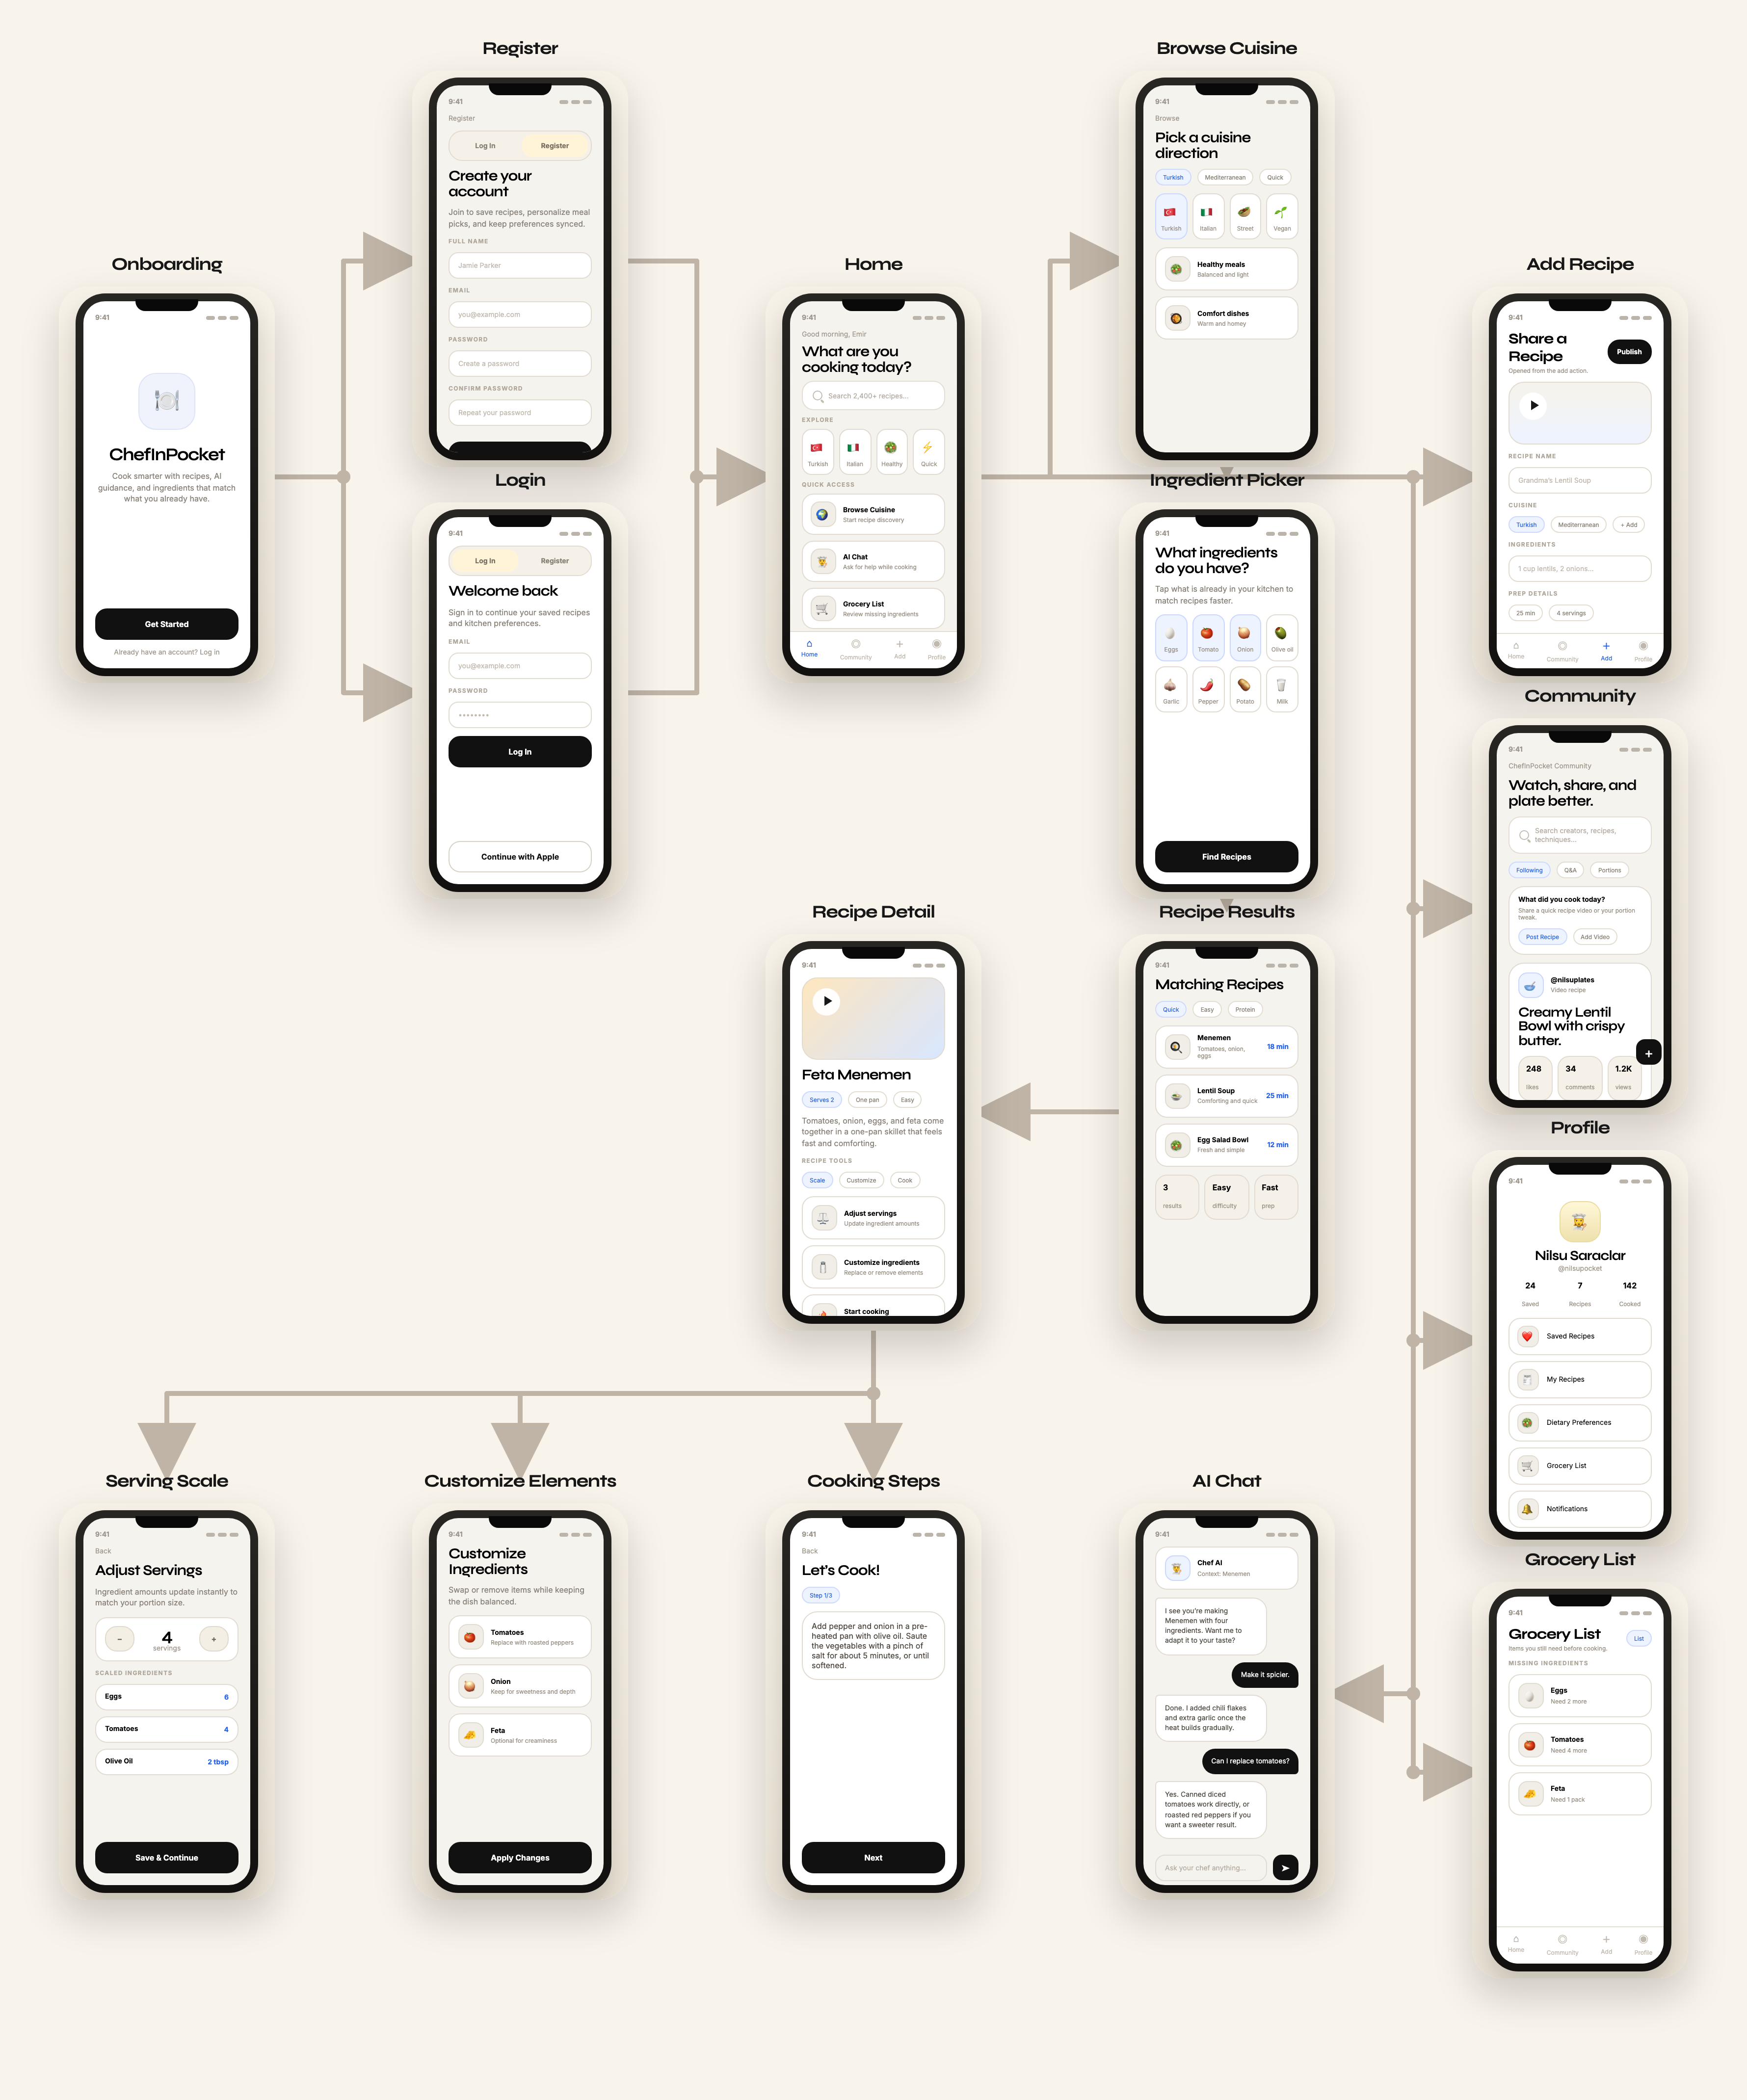
\includegraphics[width=\textwidth]{ChefInPocket_Wireflow_Board.png}
  \caption{ChefInPocket — Full Wireflow Board (16 screens, including navigation links)}
\end{figure}

The application flow is \textbf{intentionally branched}—only transitions that make sense are presented.

\begin{enumerate}
  \item \textbf{Access Branch:} Onboarding $\rightarrow$ Register or Login $\rightarrow$ Home.
  \item \textbf{Discovery Branch:} Home $\rightarrow$ Browse Cuisine $\rightarrow$ Ingredient Picker $\rightarrow$ Recipe Results $\rightarrow$ Details about the recipe.
  \item \textbf{Recipe Tool Branch:} Recipe Detail $\rightarrow$ Serving Size, Customizing Ingredients, and Cooking Steps.
  \item \textbf{Direct Home Branch:} Home (bottom nav) $\rightarrow$ AI Chat, Grocery List, Add Recipe, Community, Profile.
\end{enumerate}

\subsection*{Navigation Components Used}
\begin{itemize}
  \item \textbf{Segmented Control} — A toggle for registering or logging in to switch between authentication flows.
  \item \textbf{Contextual Pills} — The Cuisine, Recipe Detail, and Recipe Results pages all use pill chips for sub-views.
  \item \textbf{Back Label} — The Serving Scale and Cooking Steps let you go back on the screen.
  \item \textbf{Floating Action Button} — The Community screen has a "+" FAB button for easy posting.
\end{itemize}

%% ══════════════════════════════════════════════════════════════
\section{Wireframe Screens}

%% ── 1. AUTH FLOW ─────────────────────────────────────────────────────────────
\subsection{Authentication Flow}

\medskip
\noindent
\sblock{screenshots/01-onboarding.png}{1}{Onboarding}{%
  This is the initial page that new users see. It has two buttons: "Get Started" and "Log In."}
\hfill
\sblock{screenshots/02-register.png}{2}{Register \textnormal{{\tiny(Input Form )}}}{%
  Account creation form with a segmented control toggling between Register and Log In.}
\hfill
\sblock{screenshots/03-login.png}{3}{Login}{%
  Email and password boxes for returning users, as well as a "Continue with Apple" option.}

%% ── 2. HOME ──────────────────────────────────────────────────────────────────
\subsection{Home Screen}

\begin{minipage}[c]{0.34\textwidth}
  \centering
  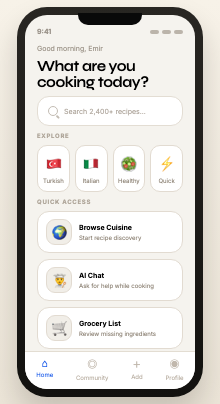
\includegraphics[width=0.80\linewidth]{screenshots/04-home.png}\\[5pt]
  {\small\bfseries Screen 4 — Home}
\end{minipage}%
\hfill
\begin{minipage}[c]{0.62\textwidth}
  \centering
  The main part of the app is the "central hub," which has the recipe search bar, cuisine category grid, quick-access cards, and bottom navigation bar, all of which can be reached with only two touches.
\end{minipage}

\medskip

%% ── 3. DISCOVERY FLOW ────────────────────────────────────────────────────────
\subsection{Recipe Discovery Flow}

\medskip\noindent
\sblock{screenshots/05-browse-cuisine.png}{5}{Browse Cuisine}{%
  A pill-row filter and a 4-column icon grid let you explore different types of food and categories.}
\hfill
\sblock{screenshots/06-ingredient-picker.png}{6}{Ingredient Picker \textnormal{{\tiny(Input Form )}}}{%
  Tag-based multi-select interface; touching on ingredients highlights them, and \emph{Find Recipes} starts the search.}
\hfill
\sblock{screenshots/07-recipe-results.png}{7}{Recipe Results}{%
  The recipe list was sorted by name, cook time, and pill criteria (Quick, Easy, and Protein).}

%% ── 4. RECIPE DETAIL + TOOLS ─────────────────────────────────────────────────
\subsection{Recipe Detail and Tools}

\medskip\noindent
\sblock{screenshots/08-recipe-detail.png}{8}{Recipe Detail}{%
  This is a single-recipe portal with a hero media, a title, pills, and three tool actions: Scale, Customize, and Cook.}
\hfill
\sblock{screenshots/09-serving-scale.png}{9}{Serving Scale}{%
  The stepper control ($-$/+) changes the number of servings and figures out how much of each ingredient to use in real time.}
\hfill
\sblock{screenshots/13-customize.png}{13}{Customize Elements}{%
  The ingredient replacement interface shows a different option for each row and lets you save the changes with \emph{Apply Changes}.}

\medskip

%% Cooking Steps – side-by-side with vertically centred description
\noindent
\begin{minipage}[c]{0.34\textwidth}
  \centering
  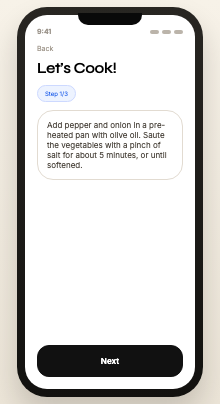
\includegraphics[width=0.80\linewidth]{screenshots/14-cooking-steps.png}\\[5pt]
  {\small\bfseries Screen 14 — Cooking Steps}
\end{minipage}%
\hfill
\begin{minipage}[c]{0.62\textwidth}
  \centering
  Step-by-step guided cooking mode showing one step at a time; lets you follow the recipe without getting lost.
\end{minipage}

\medskip

%% ── 5. UTILITY SCREENS ───────────────────────────────────────────────────────
\subsection{Utility Screens}

\medskip\noindent
\sblock{screenshots/10-ai-chat.png}{10}{AI Chat}{%
  The context-aware conversational assistant shows the active recipe badge, AI bubbles on the left, and user bubbles on the right.}
\hfill
\sblock{screenshots/11-grocery-list.png}{11}{Grocery List}{%
  A missing-ingredient tracker with an icon and quantity rows that shoppers tick off as they go.}
\hfill
\sblock{screenshots/12-add-recipe.png}{12}{Add Recipe \textnormal{{\tiny(Input Form )}}}{%
  Form for publishing recipes that has a title, cuisine pills, an ingredients section, and a \emph{Publish} button.}

%% ── 6. SOCIAL + PROFILE ──────────────────────────────────────────────────────
\subsection{Social and Profile}

\medskip\noindent
\sblock{screenshots/15-community.png}{15}{Community}{%
  A social feed with pill filters, a composer card, recipe cards with interaction stats, and a \texttt{+} FAB.}
\hfill
\sblock{screenshots/16-profile.png}{16}{Profile}{%
  The personal account hub has stat tiles, a settings menu, and a Log Out button.}
\hfill
\begin{minipage}[t]{0.30\textwidth}\end{minipage}

\end{document}